\documentclass{article} % For LaTeX2e
\usepackage{nips15submit_e, times}
\usepackage{hyperref}
\usepackage{url}
\usepackage{amsmath}
\usepackage{amsfonts}
\usepackage{amssymb}
\usepackage{color}
\usepackage{cite}
\usepackage{epsfig, graphics}
\usepackage{bm}
\usepackage{enumitem}

\title{Predicting Movie Rating with Parallel Stochastic Gradient Descent \& Hybrid Matrix Factorization}

\author{
Kanit Wongsuphasawat, Supasorn Suwajanakorn \\
% \thanks{ Use footnote for providing further information
% about author (webpage, alternative address)---\emph{not} for acknowledging
% funding agencies.} \\
Computer Science \& Engineering\\
University of Washington\\
\texttt{\{supasorn,kanitw\}@cs.washington.edu} \\
}

% The \author macro works with any number of authors. There are two commands
% used to separate the names and addresses of multiple authors: \And and \AND.
%
% Using \And between authors leaves it to \LaTeX{} to determine where to break
% the lines. Using \AND forces a linebreak at that point. So, if \LaTeX{}
% puts 3 of 4 authors names on the first line, and the last on the second
% line, try using \AND instead of \And before the third author name.

\newcommand{\fix}{\marginpar{FIX}}
\newcommand{\new}{\marginpar{NEW}}
\newcommand{\todo}[1]{\textcolor{red}{TODO: #1}}
\newcommand{\red}[1]{\textcolor{red}{#1}}
\newcommand{\U}{U}
\newcommand{\M}{M}
\newcommand{\kernel}{K}

\nipsfinalcopy % Uncomment for camera-ready version

\nipsfinalcopy % Uncomment for camera-ready version

\begin{document}

\maketitle



\section{Problem}

Our goal is to predict movie ratings for each user based on previous ratings
and movie metadata including genres and user-provided tags.

\todo{finish writing intro}
To address cold-start problem, we formulate


Specifically, we implement a learning model based on matrix
factorization~\cite{koren:matrix} that addresses the following problems:

\textbf{1) Cold-Start Problem.}
A common problem for matrix factorization-based method for collaborative
filtering is the inability to address unseen items (movies in our case) or
users.  We address this problem by using a hybrid model combining matrix
factorization and content-based filtering techniques using metadata as
features. To address high dimensionality, we compress tags' feature vectors
using hash-kernel techniques~\cite{shi:hashkernels}.

\textbf{2) Run-time Performance.}
We aim to explore parallelization techniques and frameworks that enable fast
learning algorithm.  In our initial work, we experiment with a simple
interference-free parallelization scheme for stochastic gradient descent
(SGD) which avoids work overriding and can simultaneously utilize all
available cores. We plan to implement and compare SGD on a distributed
framework such as GraphLab.

% We plan to compare our method with Hogwild method by Niu et al.~\cite{niu:hogwild} that uses a shared-memory model without locks to eliminate the locking overhead.



\section{Dataset \& Preprocessing}

We use the MovieLens 20M\footnote{http://grouplens.org/datasets/movielens/}
as our benchmark dataset.  The dataset contains the following features:

\begin{itemize}[leftmargin=15pt]
	\item Over 20 million ratings for 27,278 movies by 138,493 users ($n_u$).
	0.5\% of the rating matrix $R$ has non-zero values.
	\item Genres of each movie, given as a set of genres associated with each
movie. There are 19 unique genres ($n_g$).
	\item 65,564 user-provided tags (37,896 unique tags), such as ``dark hero'', ``bollywood'',
	``conspiracy theory''.  We remove space and symbols for each tag to remove duplicate entities.
	\item All users included in the data have rated at least 20 movies.
\end{itemize}

Our model will be evaluated on both the cold-start problem and the standard
prediction problem (in which we predict unknown ratings for already-seen
movies in the training set). To achieve that, we generated two datasets from the
rating matrix R (of rank $n_u \times n_m$):

\textbf{1) Training and test data set for the standard problem ($D_s$).}
For the standard problem, we obtain a test set by taking out 20\% of all the
ratings from the rating matrix and use the remaining for training.
Due to our limited computational resources and time, it is infeasible to
perform a cross-validation on the full training set, so we divide a subset
of the training data into 4:1 split as a small training and validation set
for determining hyper-parameter.  Once all hyper-parameters are learned, we
re-train our model on the full training set (i.e. 80\% of original data) and
evaluate on the test set.

\textbf{2) Training and test data set for the cold-start problem ($D_c$).}
For the cold-start problem, we obtain a test set by taking out 20\% of   the
{\em columns} from the rating matrix and use the remaining for training. This
assures that all the ratings of each movie in the test set have not been
included for model learning.   For cross-validation, we further split the
training set, re- train the model on the full training set, and evaluate on
the test set akin to the standard data set.



\section{Formulation}

\subsection{Pure Matrix Factorization}

We first formulate rating prediction task as a pure matrix factorization
problem  where $r_{um}$ is the user $u$'s rating for movie $m$ while $L_u,
R_m \in \mathbb{R}^k$ are $k$ dimensional latent vectors associated with
user $u$ and movie $m$.

The objective function is
\begin{align}
\min_{L, R} \frac{1}{2}\sum_{r_{um}} \left\{(L_u \cdot R_m - r_{um})^2\right\}
	+ \frac{\lambda_u}{2}\|L\|^2_F + \frac{\lambda_m}{2}\|R\|^2_F \label{eq:mf}
\end{align}

where $\lambda_u$ and $\lambda_m$  are regularization parameters for each latent matrix.

\subsection{Hybrid Matrix Factorization}

In MovieLens data, each movie $m$ has a set of genres and user-specified
tags. This implicit information is useful in scenario where we try to
predict ratings for unobserved movies that have similar tags to the existing
ones and can be used in a feature-based model to complement the prediction.

For each movie, we model the genres a boolean vector $\bm{g_m} \in
\{0,1\}^{19}$ and tags count vector $\bm{t_m} \in \mathbb{N}_0^{465,564}$ where
$t_m^j$ represents the number of times that movie $m$ is tagged by tag $j$.  To
compress the tag vector, we use hash kernel to project each
$\bm{t_m}$ to a 40-dimensional kernel vector $\kernel(\bm{t_m})$ using hash
function $h$ and $\xi$ sign hash function.
\begin{align}
	\kernel_i(\bm{x}) &= \sum_{j:h(j)=i} \xi(j) \bm{x_j}
\end{align}
\begin{center}
where $h: X \rightarrow \{1, ..., 40\}$ and $\xi: X \rightarrow \{1,-1\}$.
\end{center}

We then normalize the kernel projection using $L_0$ norm.
\begin{align}
	\hat{\kernel}(\bm{t_m}) = \frac{\kernel(\bm{t_m})}{\|\kernel(\bm{t_m})\|_0}
\end{align}

After compression, we can model feature vector for each movie.
\begin{align}
	\phi(m) = [\bm{g_m}\ \ \hat{\kernel}(\bm{t_m})]
\end{align}

With these features, we model the interaction as a dot product $w \cdot
\phi(m)$ where $w$ is a weight vector associated with the feature vector.
However, the weight might vary across different users and movies. Different
users might have varied preference for each movie genre and tag. For
example, one might prefer action movies while another might prefer dramas.
Similarly, different movie might have varied interaction with its own
feature. For example, consider a scenario where we try to predict ratings of
a user $u$ for two different movies where one of the movies stars a very
famous actress and the other stars a less well-known set of casts. One can
imagine that people may pay less attention to genres if a movie stars their
favorite actors/actresses and more attention when they do not know much
about the film casts. This suggests that movie-specific biases can be
beneficial for modeling this kind of behavior.  Thus we define the weight
vector $w = w_u + w_m$ where $w_u$ is a weight vector associated with user
$u$ and  $w_m$ is a weight vector associated with movie $m$

Moreover, since part of the observed variation in the ratings is attributed
to similar systematic biases \cite{koren:matrix} where certain users tend to
rate, on average, higher (or lower) than their peers or certain movies tend
to be highly rated, we incorporate user- and movie-specific bias terms
($b_u$ and $b_m$) in the rating in the final prediction so that the dot
product of the movie and user latent variables instead describes the
deviation from the user/movie's mean rating.

A true first-order approximation of these systematic biases includes a
global bias or weight shared by all users. However, we use a slightly
different approximation that folds the global bias into individual biases so
that learning can be done efficiently due to the ability to  partition the
data into independent sub-problems. This allows sequential-consistent
learning algorithms to run with fewer blocking operations or enable other
bulk or distrubuted synchronization strategies such as Distributed
Stochastic Gradient Descent (DSGD)~\cite{gemulla2011large}, or
NOMAD~\cite{yun2013nomad}.

Our final unified collaborative filtering model combines matrix
factorization with a feature-based learning to address cold-start problem:

\begin{multline}
\min_{L, R, b_u, b_v, w_u, w_m} \frac{1}{2}\sum_{r_{um}} \left\{(L_u \cdot R_m + (w_u + w_m) \cdot \phi(m) + b_u + b_m - r_{um})^2\right\}\\ + \frac{\lambda_u}{2}\|L\|^2_F + \frac{\lambda_m}{2}\|R\|^2_F + \frac{\lambda_{w_u}}{2}\sum_u\|w_u\|^2_2 + \frac{\lambda_{w_m}}{2}\sum_m\|w_m\|^2_2\label{eq:main}
\end{multline}

where
\begin{itemize}
	\item $L_u, R_m \in \mathbb{R}^k$ are $k$ dimensional latent vectors associated with user $u$ and movie $m$.
	\item $w_u,w_m \in \mathbb{R}^{dim(\phi)}$ are latent feature weights.
	\item $b_u, b_m \in \mathbb{R}$ are individual and movie-specific biases for the rating $r_{um}$.
	\item $\phi(m)$ is a feature containing movie genres and user-specified tags.
	\item $\lambda_u$, $\lambda_m$, $\lambda_{w_u}$, and $\lambda_{w_m}$ are regularization parameters.
\end{itemize}

\section{Learning}

\textbf{Update Equation.}   We use stochastic gradient descent to optimize
Equation $\ref{eq:main}$. The update equations for the latent variables given
a rating $r_{um}$ are:

\begin{align}
L_u^{i+1} &= L_u^{i} - \eta ( \epsilon_{um} R_m  + \lambda_u L_u^i)\\
R_m^{i+1} &= R_m^{i} - \eta ( \epsilon_{um} L_u  + \lambda_u R_m^i)\\
w_u^{i+1} &= w_u^{i} - \eta ( \epsilon_{um} \phi(m) + \lambda_{w_u} w_u^i)\\
w_m^{i+1} &= w_m^{i} - \eta ( \epsilon_{um} \phi(m) + \lambda_{w_m} w_m^i)\\
b_u^{i+1} &= b_u^{i} - \eta \epsilon_{um}\\
b_m^{i+1} &= b_m^{i} - \eta \epsilon_{um}
\end{align}
where
\begin{align}
	\epsilon_{um} &= L_u \cdot R_m + (w_u + w_m) \cdot \phi(m) + b_u + b_m - r_{um}
\end{align}

\begin{center}
and $\eta$ is the learning rate.
\end{center}

\textbf{Stopping criteria.}   We iterate on the stochastic gradient descent
for a maximum of 30 rounds (20 rounds for the validation phase--due to
computing limitation)   or if the changes in rmse falls below 0.005.



\section{Parallelization Scheme and Implementation}

\subsection{GraphLab}

We use GraphLab Create \todo{version}

\subsection{NOMAD}

\subsection{DSGD}



\section{Experiments}

$\eta=0.05$

\subsection{Performance}

We spend equal amount of time optimizing both parallelization scheme.

\subsection{Hyperparameter Optimization}

We run a grid search to optimize hyperparameters for both pure and hybrid
matrix factorization. We search over $k \in \{5, 10, 20\}$, $\lambda \in \{0,
0.001, 0.01, 0.1, 1, 10\}$ for both formulation and $\lambda_m \in \{0,
0.001, 0.01, 0.1, 1, 10\}$ for the hybrid model.

Due to resource limitation, we search for parameter using a subset of 1 million


We also run only the NOMAD algorithm as it
has been shown in the previous section that it has the highest performance.

Figure~\ref{fig:gridsearch} shows resulting $rmse_{validate}$ from the grid search.
For both formulation, the optimal $rmse_{validate}$ are obtained when
$k=20$, $\lambda=0.1$ and $\lambda_w=1$ (for the hybrid model).

\begin{figure}[h]
\centering
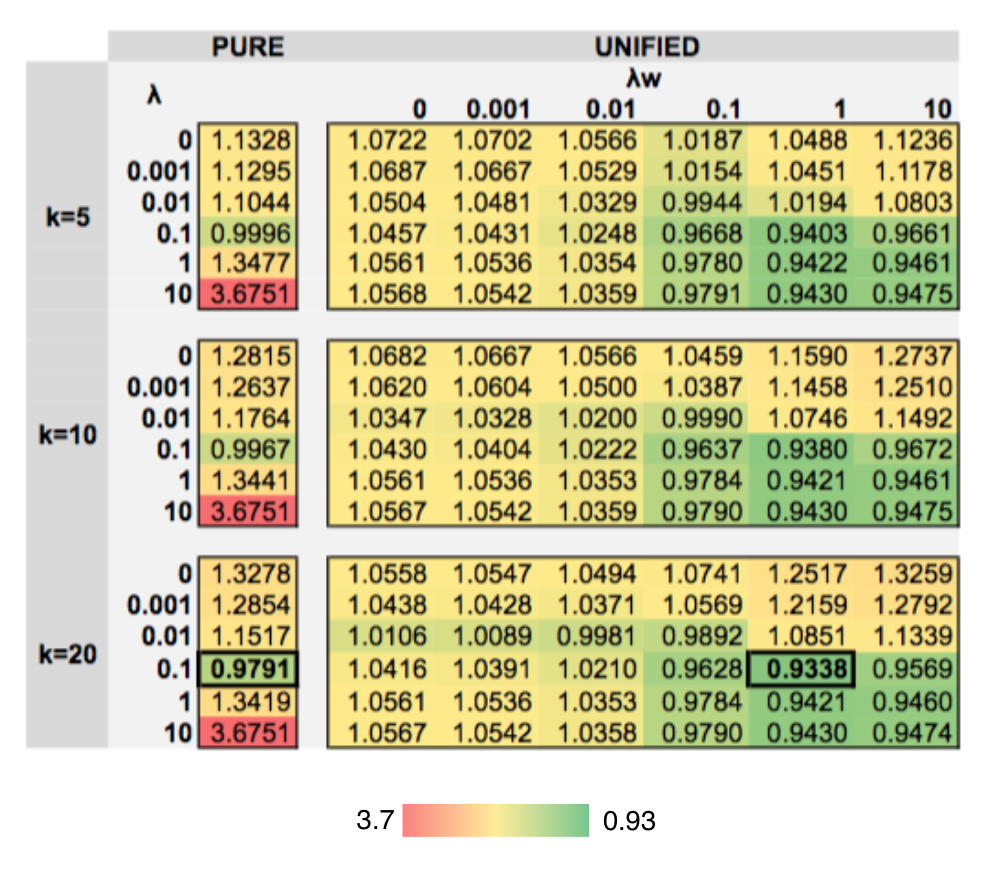
\includegraphics[width=3.5in]{grid-search.png}
\caption{\label{fig:gridsearch} Heatmap Table showing $rmse_{validate}$ from
running grid search for different parameters $k$, $\lambda$, $\lambda_m$ for
both hybrid and pure MF using 1M subset of the training data.  Lower $rmse$
values are shown in green while high values are shown in red.  Optimal $rmse$
for each formulation are highlighted with a bold text and thick border.}
\end{figure}




\subsection{Experimenting with $D_n$}

- grid parameter
- plot rmse validation across parameter
- report final rmse test with two algorithm -- bar chart

\subsection{Experimenting with $D_{cs}$}



\section{Conclusion}


\bibliographystyle{abbrv}
\bibliography{paper_supasorn_kanitw}{}
\end{document}

